\subsection{Results}

\nb{The preemption rate is computed as $\frac{scheduler.preempted}{lcm}$ if the system is schedulable with the current configuration, $\frac{scheduler.preempted}{scheduler.i}$ otherwise (for schedulable systems $lcm = scheduler.i$).}


\ref{fig:stu:au} shows an exponential decrease of the schedulability rate in $u$ as well as a nearly linear increase of preemption rate with constant factor $0.1$.

\begin{figure}
	\centering
	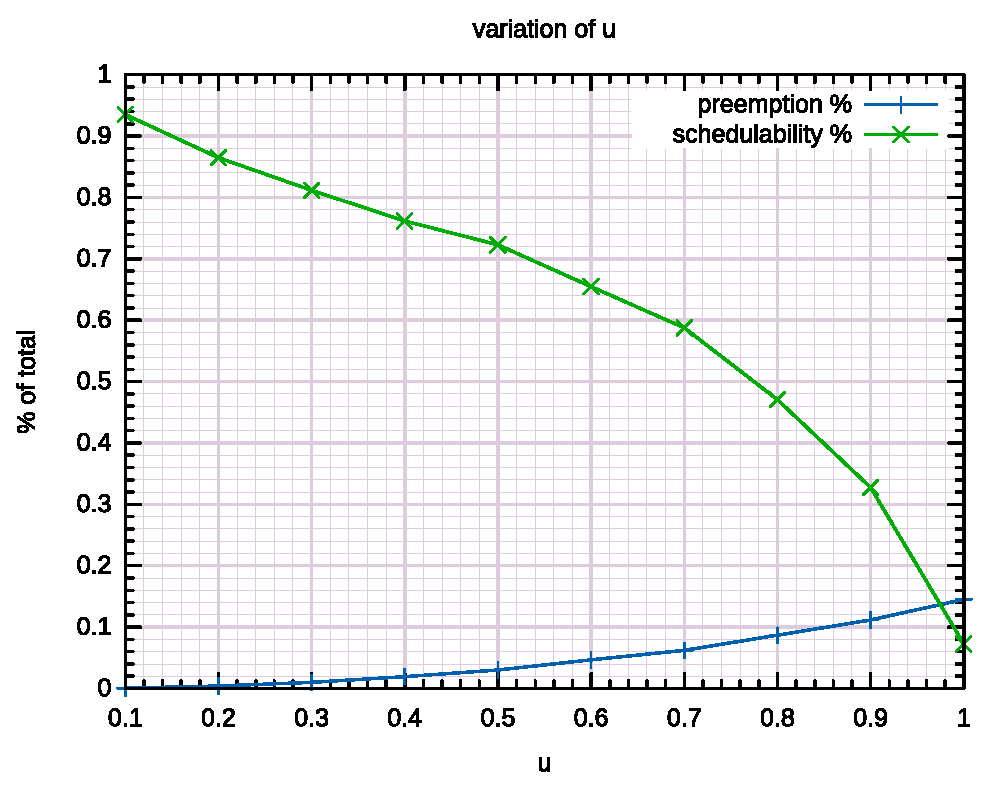
\includegraphics[width=0.8\textwidth]{../gnuplot/eps/1}
	\caption{\label{fig:stu:au} Schedulability an Preemption rate depending on $u$}
\end{figure}


\ref{fig:stu:ad} shows a nearly linear decrease of the schedulability rate in $\Delta_r$ with constant factor $0.02$ as well as a negative exponential decrease of the preemption rate.

\begin{figure}
	\centering
	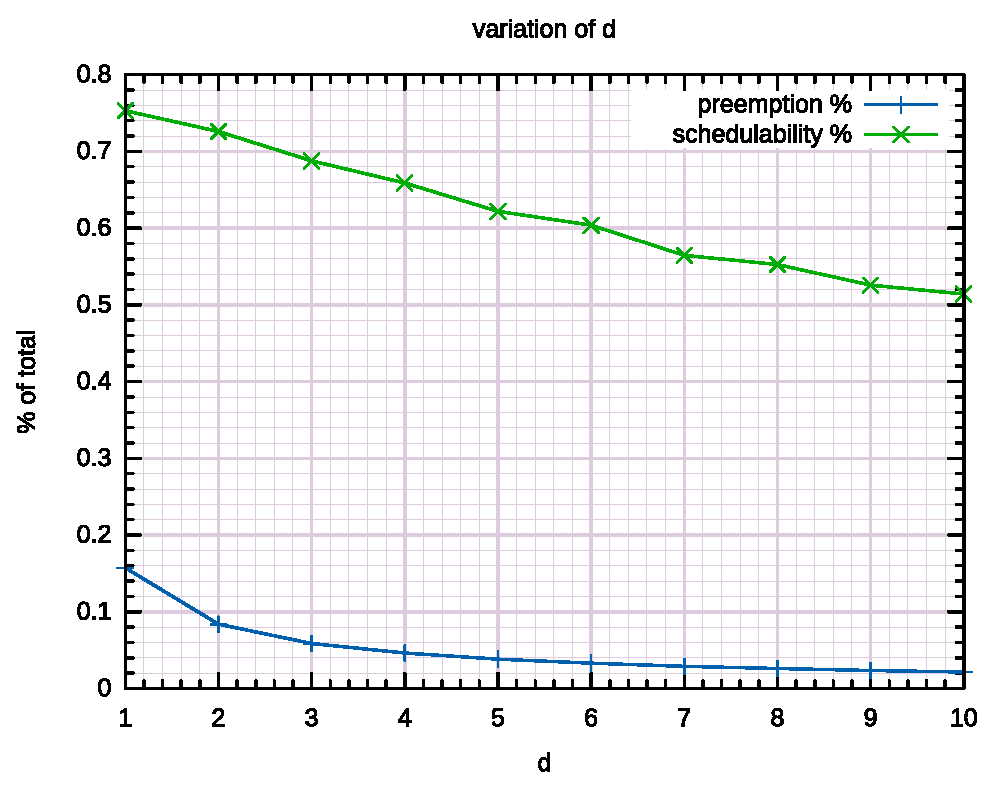
\includegraphics[width=0.8\textwidth]{../gnuplot/eps/2}
	\caption{\label{fig:stu:ad} Schedulability an Preemption rate depending on $\Delta_r$}
\end{figure}

\ref{fig:stu:an} shows a nearly linear decrease of the schedulability rate in $n$ as well as a linear increase of the preemption rate. This result is probably not exploitable since the range of $n$ value is not wide enough.

\begin{figure}
	\centering
	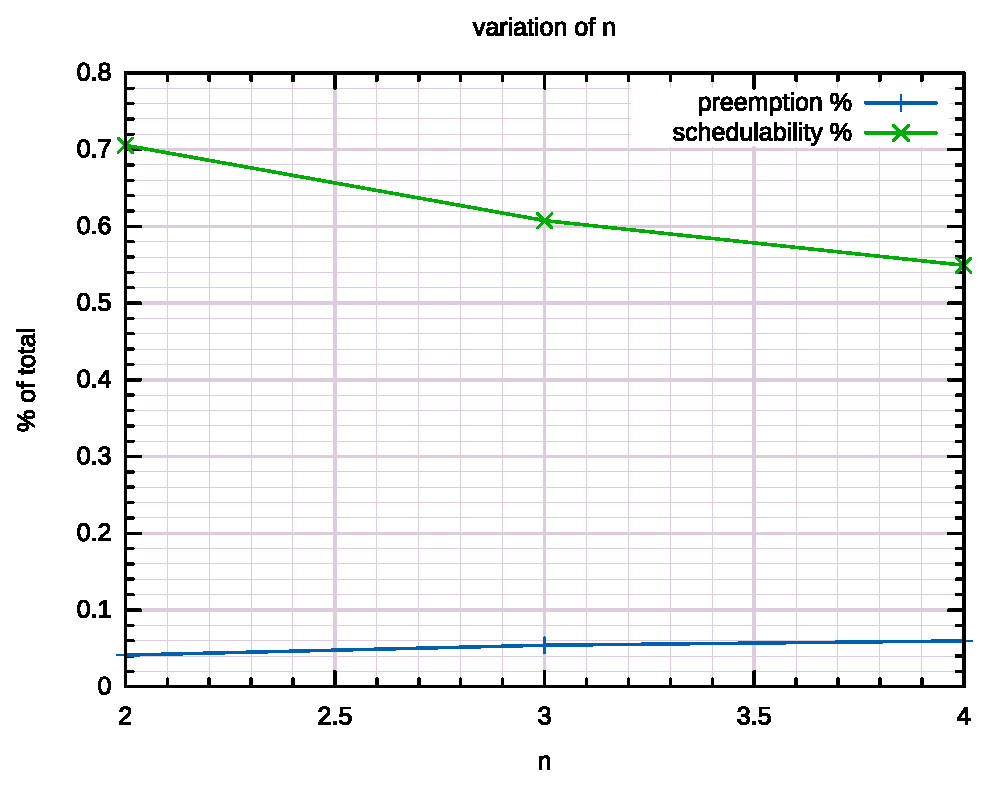
\includegraphics[width=0.8\textwidth]{../gnuplot/eps/3}
	\caption{\label{fig:stu:an} Schedulability an Preemption rate depending on $n$}
\end{figure}

\ref{fig:stu:4p} shows the influence of $u$ and $\Delta_r$ on the preemption rate ($n = 4$).

\begin{figure}
	\centering
	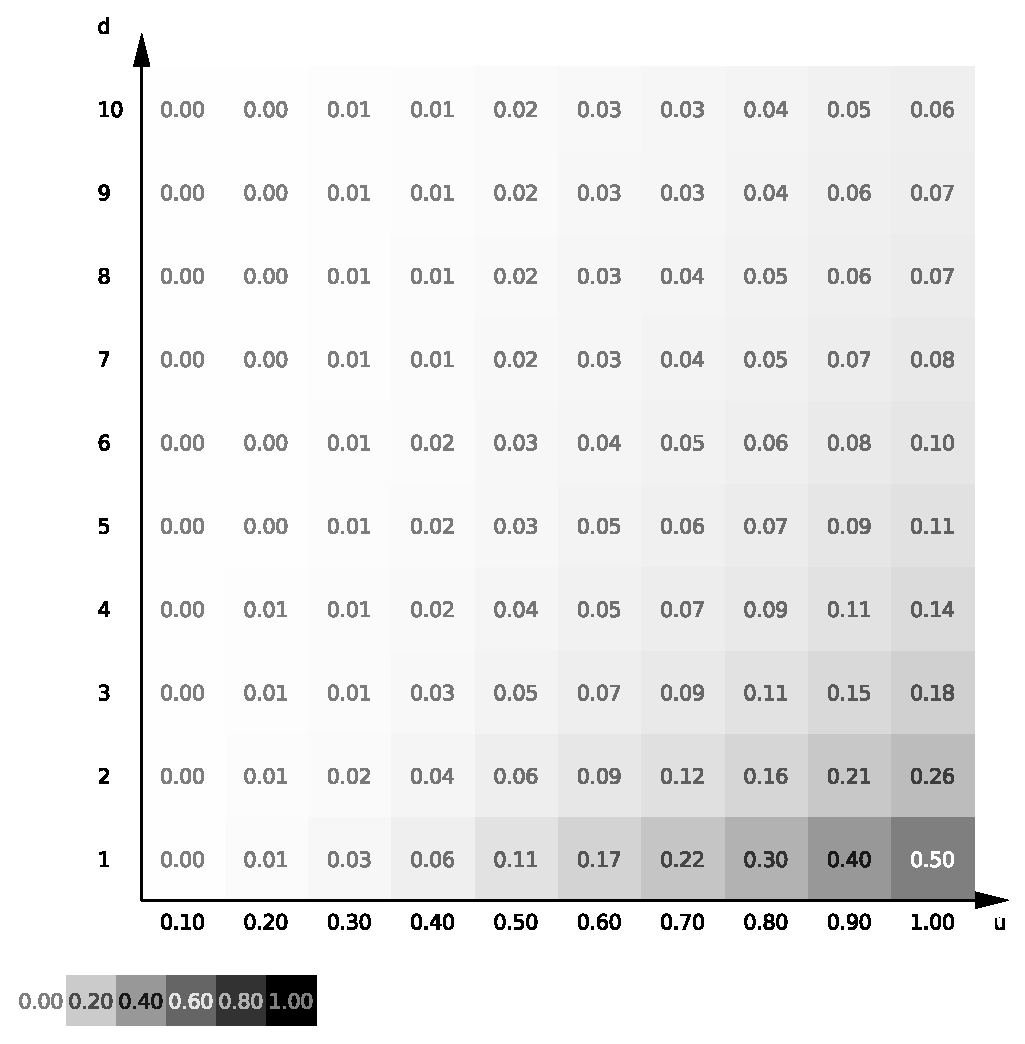
\includegraphics[width=1\textwidth]{../mean/eps/4p}
	\caption{\label{fig:stu:4p} Preemption rate for $n = 4$}
\end{figure}

\ref{fig:stu:4s} shows the influence of $u$ and $\Delta_r$ on the schedulability rate ($n = 4$).

\begin{figure}
	\centering
	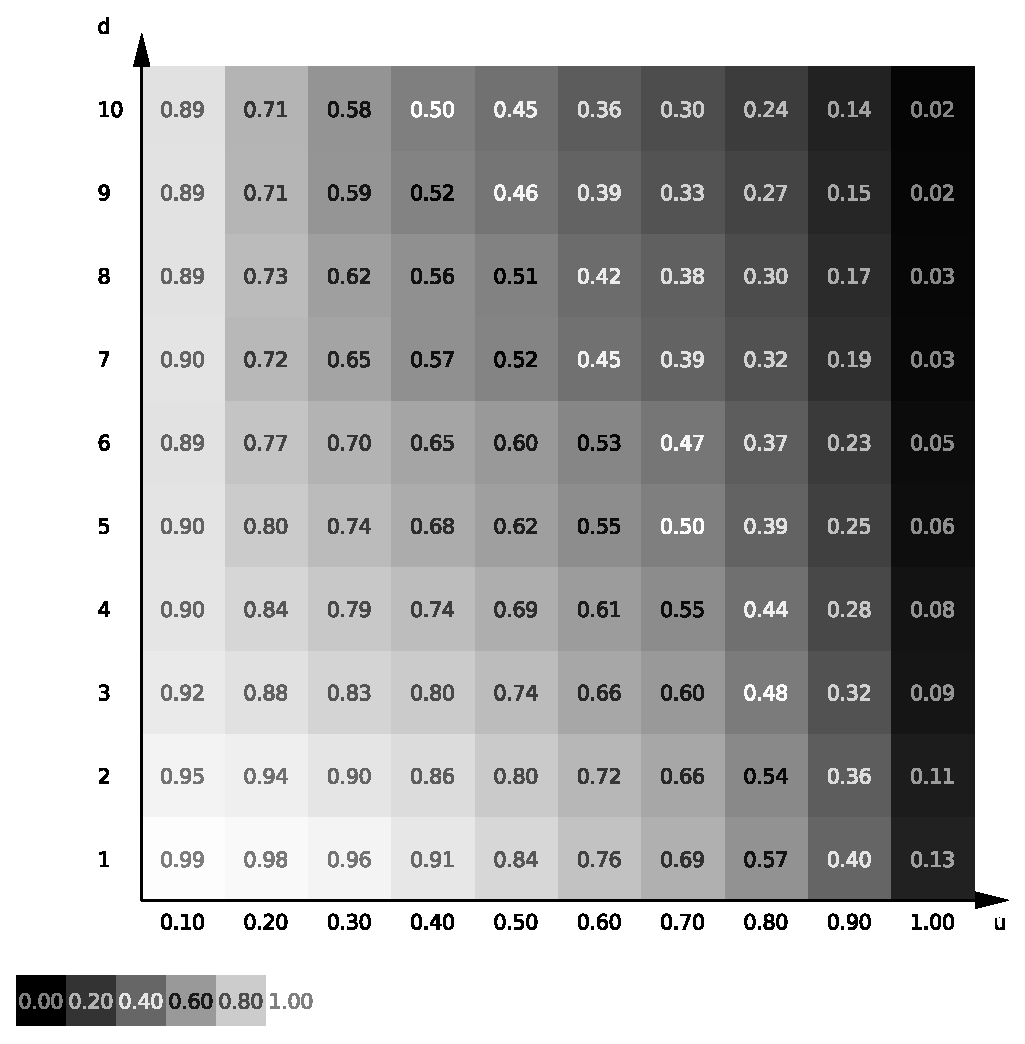
\includegraphics[width=1\textwidth]{../mean/eps/4s}
	\caption{\label{fig:stu:4s} Schedulability rate for $n = 4$}
\end{figure}
